\begin{sol}
    \begin{enumerate}[label=\textbf{(\alph*)}]
        \item 
        Since energy doesn't stuck in anywhere we can write conservation of energy for a cylinder height $h$ and radius $r$ : 
        $$-\kappa 2\pi r\cancel{h}\dv{T}{r}=\qty(I\frac{\pi r^2}{\pi R^2})^2\rho\frac{\cancel{h}}{\pi r^2}$$
        so we can seperate and integrate. we get $T=-\frac{I^2r^2\rho}{4\pi^2 R^4\kappa}+\mathcal{C}$. We can find constant from $T(r=R)=T_0$. So 
        $\mathcal{C}= T_0+\frac{I^2\rho}{4\pi^2 R^2\kappa}$. Finally $$T(r)=T_0+\frac{I^2\rho}{4\pi^2 R^2\kappa}\qty(1-\frac{r^2}{R^2})$$
        \item
        The magnetic force acts perpendicular to velocity. and electric fieald is always acts along radial. So first accelerates and at the same time it rotates with increasing radius. and after $v_r$ being 0 electric force try to slow it down and this proccess happens over and over again.
        \begin{center}
        
            \incfig{drawing}
        \end{center}
        \item
        Since there're two cylinders with potential of $-V$ and 0 we can assume that system is a cylinderic condenstor. So we can find $E$ field inside of condensator.  
        $$\int_a^b \frac{\lambda}{2\pi \veps_0 r}\dd r=V$$ we can find the formula for $E$ with taking cylinderic gaussian surface. And substituting $\lambda$ to equation of $E$ we get that $E=\frac{V}{\ln(\frac{b}{a})r}$. 

        Let $v_r$ and $v_z$ will be radial and along wire components of velocity respectively.The magnetic fieald of infinite wire is $B=\frac{\mu_0I}{2\pi r}$. Using right hand rule we see that magnetic force due radial velocity acts on parallel  velocity. We can write force equation for $v_z$: $$m\dv{v_z}{t}=e\frac{\mu_0I}{2\pi r}v_r$$
        multipliying both sides by $\dd t$ and using $v_r\dd t=\dd r$ and integrating we get $$mv_z=e\frac{\mu_0I}{2\pi}\ln\frac{r_{max}}{a}$$ We can write work-energy equation for electron. since magnetic force doesn't change the velocity we can write 
        \begin{align*}
        &\int_a^{r_{max}}e\frac{V}{\ln(\frac{b}{a})r}\dd r=\frac{mv_z^2}{2}\\
        &2e\frac{V}{\ln(\frac{b}{a})}\ln\frac{r_{max}}{a}=mv_z^2
        \end{align*}
        At maximum distance there will not be radial speed. So if we square our force equation and substitute $mv_z^2$ we get
        $$2\cancel{e}\frac{V}{\ln(\frac{b}{a})}\cancel{\ln\frac{r_{max}}{a}}=\frac{e^{\cancel{2}}\mu_0^2I^2}{4\pi^2m}\qty(\ln(\frac{r_{max}}{a}))^{\cancel{2}}$$
        And $r_{max}$ is $$r_{max}=a\exp(\frac{8\pi^2mV}{\ln\frac{b}{a}e\mu_0^2I^2})$$
        \item
        
        \item
        We  didn't succeed at previous part so we are gonna show graph of non-relavitistic case  
        \begin{center}
            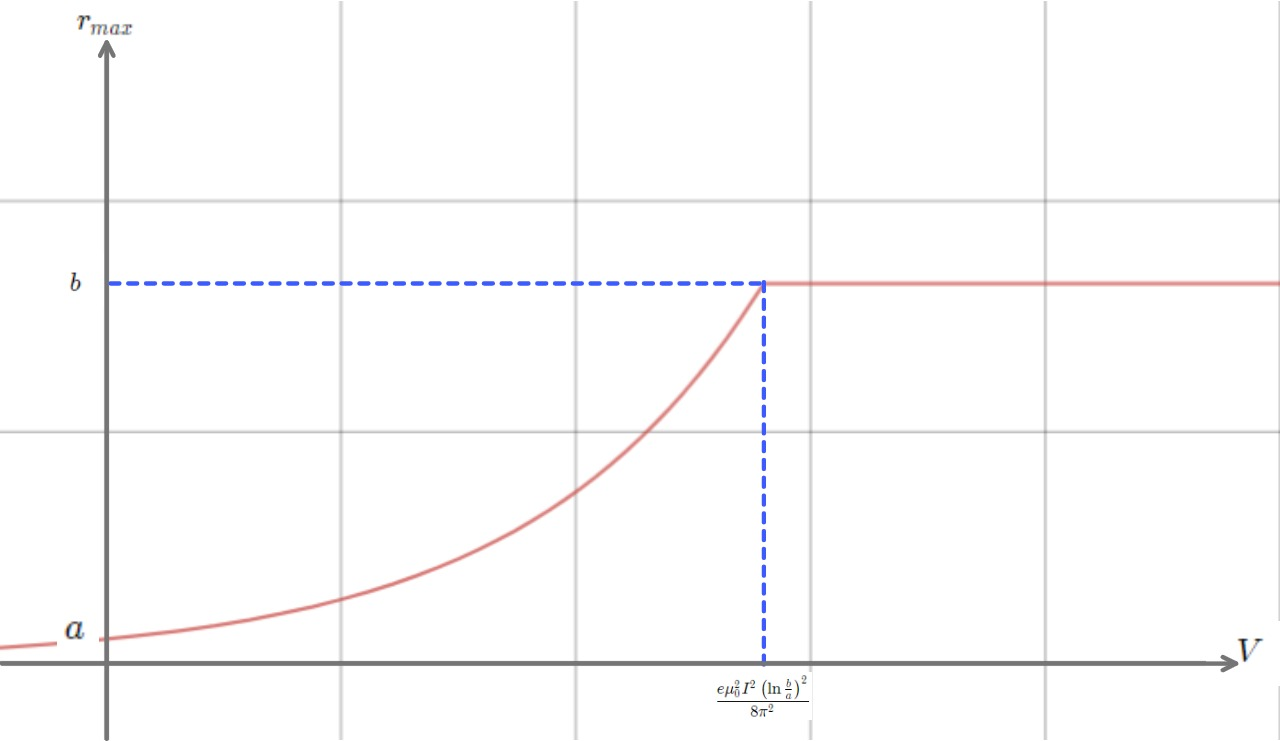
\includegraphics[width=0.4\textwidth]{image.jpg}
        \end{center}
    \end{enumerate}
\vspace{15mm}
\end{sol}